%% \chapter{Simulationen von kristallinem und amorphem Silizium}
%% \label{appendix_silicon}

%% Die Bindungslängen für verschiedene Parametrisierungen wurden direkt aus der ersten Spitze in der radialen Verteilungsfunktion für einen Silizium-Kristall nach einer thermischen Relaxierung ermittelt und in Abbildung~\ref{fig:sisibondlengths} zusammen gefasst.
%% Für die \pot{newsome}-Parametrisierung ergibt sich durch Aufspaltung der Hauptbindungslänge eine zusätzliche RDF-Spitze vor der eigentlichen Bindungslänge (Abbildung~\ref{fig:newsomerdf}), welche dadurch unterschätzt wird.
%% Darin zeigt sich eine Fehl\-para\-metri\-sierung des \pot{newsome}-Parametersatzes, welcher auf die Beschreibung von \ce{SiC}-Strukturen ausgelegt ist.
%% Für die anderen Parametersätze zeigen sich ansonsten gute Übereinstimmungen mit der Bindungslänge von \SI{2.3515}{\angstrom}\cite{haynes_crc_2011}.

%% \begin{figure}[p]
%%   \centering
%%   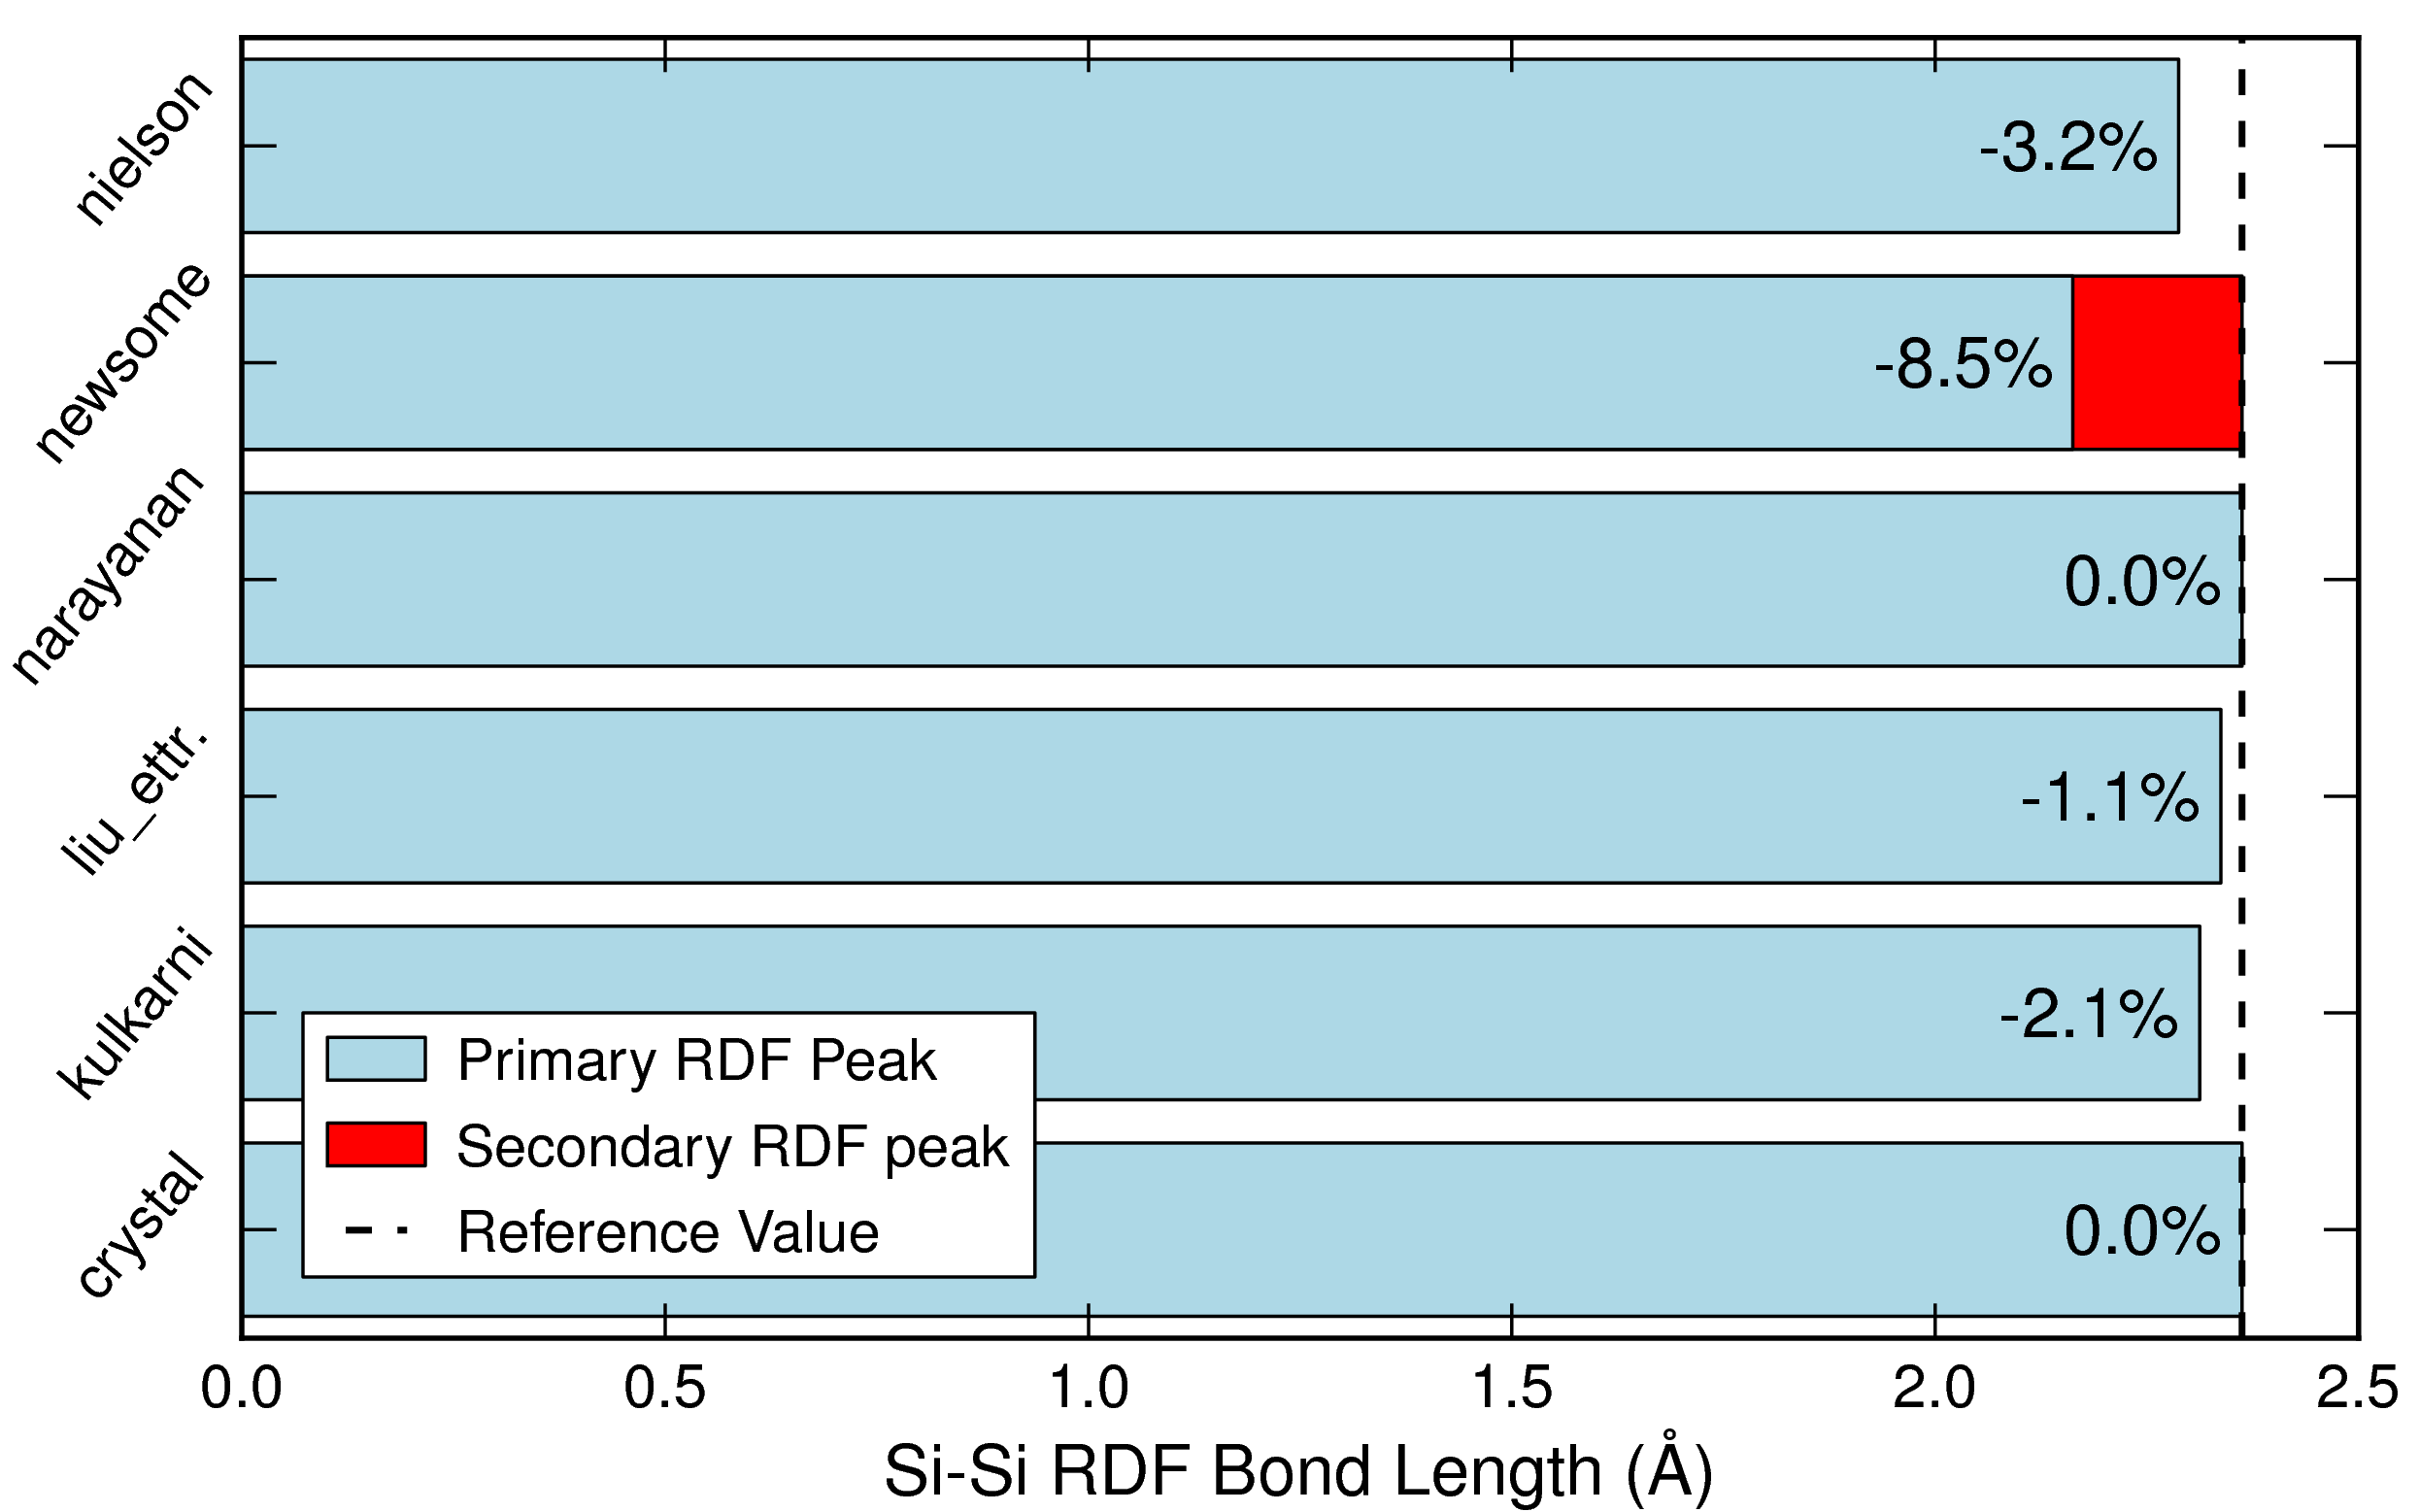
\includegraphics[width=10cm]{SiSi_npt_bondlengths}
%%   \caption{Bindungslängen von c-\ce{Si} für ReaxFF-Parametrisierungen}
%%   \label{fig:sisibondlengths}
%% \end{figure}

%% Bei Untersuchungen der RDF der Parametrisierungen hinsichtlich der Qualität der Kristalle zeigen mit Ausnahme der \pot{newsome}-Parametrisierung (Abbildung~\ref{fig:newsomerdf}) alle Parametersätze perfekte RDF-Spitzen entsprechend der kristallinen Struktur, nachdem diese sich durch thermische Bewegungen der Moleküle bei der Relaxierung verbreitert hatten.
%% Nachfolgend soll hauptsächlich die für die PVD-Simulationen genutzte \pot{kulkarni}-Parametrisierung untersucht werden, deren RDF in Abbildung~\ref{fig:kulkarnirdf}) abgebildet sind.
%% Im isotherm-isobaren Ensemble schrumpft mit ihr der Kristall zwar um \SI{2.1}{\percent}, behält seine Struktur aber ohne Einschränkung bei.


%% \section{Struktur der amorphen Schicht nach einer Parsivald-Simulation}

%% Die Rauheit der aufgewachsenen Schicht hängt stark mit der Bildung und dem Wachstum der Poren zusammen, wodurch das lineare Wachstum der Poren für einen linearen Anstieg der RMS-Rauheit sorgt.
%% Mit der Schließung der Poren ist eine schlagartige Reduktion der Rauheit zu erwarten, welcher sich gegen Ende der Simulation bereits andeutet, aber nicht mehr statt findet.
%% Simulationen über längere Zeiträume und größere Schichten sind notwendig, diesen Effekt näher zu charakterisieren

%% \begin{figure}[ht]
%%   \centering
%%   \captionsetup[subfigure]{singlelinecheck=false}
%%   \def\subfigwidth{0.48\textwidth}
%%   \begin{subfigure}[t]{\subfigwidth}
%%     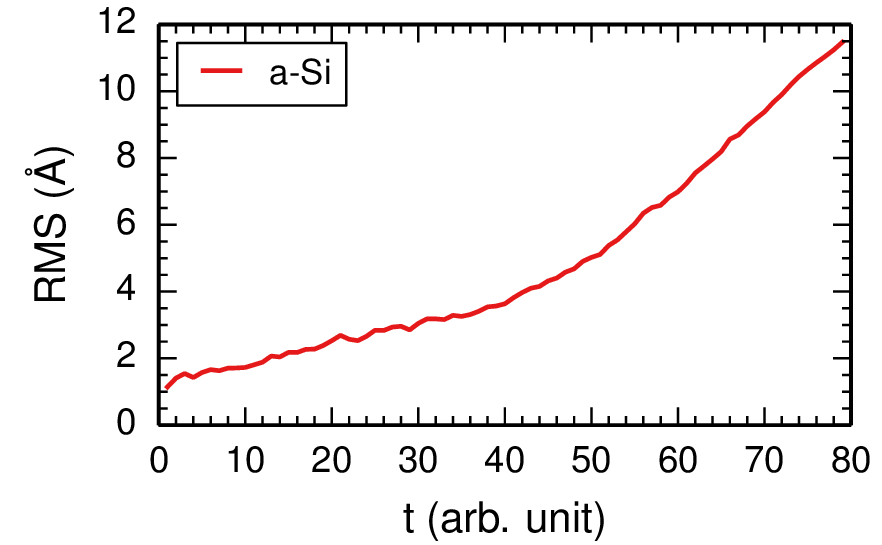
\includegraphics[width=\textwidth]{Si111_roughness}
%%     %% \subcaption{Dicke und Rauheit der Schicht}
%%     %% \label{fig:siliconresults-a}
%%   \end{subfigure}
%%   \caption{Zeitliche Entwicklung der Rauheit einer Silizium-PVD-Schicht}
%%   \label{fig:siliconroughness}
%% \end{figure}
